% Task 9: a Merkle tree. Values from checks/make_task9.py (root 34e794e7...).
\documentclass[12pt,tikz,border=6pt]{standalone}
% Shared preamble of the task figures of Lecture 6. The colours are the slide roles of Lectures 6 to 8:
%   Alice sIndigo, Eve and Mallory sPink, the message / data sViolet, a secret value sAmber,
%   Bob / the server sTeal, the digest sBrown; mechanisms neutral dark; the unknown: orange dashed.
\usepackage{lmodern}
\usepackage[T1]{fontenc}
\renewcommand{\familydefault}{\sfdefault}
\usepackage{amsmath,amssymb}
\usepackage{xcolor}
\usepackage{fontawesome5}
\usetikzlibrary{arrows.meta, calc, positioning, fit, decorations.pathreplacing, backgrounds}

\definecolor{DeepBlue}{HTML}{283593}
\definecolor{AccentOrange}{HTML}{EB5A14}
\definecolor{nInk}{HTML}{37474F}
\definecolor{nLine}{HTML}{90A4AE}
\definecolor{nLight}{HTML}{CFD8DC}
\definecolor{nFill}{HTML}{ECEFF1}
\definecolor{aExec}{HTML}{43A047}
\definecolor{aWrite}{HTML}{E53935}
\definecolor{sIndigo}{HTML}{5C6BC0}
\definecolor{sPink}{HTML}{EC407A}
\definecolor{sViolet}{HTML}{7E57C2}
\definecolor{sAmber}{HTML}{FFB300}
\definecolor{sTeal}{HTML}{26A69A}
\definecolor{sBrown}{HTML}{8D6E63}
\definecolor{sPinkText}{HTML}{C2185B}
\definecolor{sAmberText}{HTML}{A06A00}
\definecolor{sTealText}{HTML}{00796B}

\tikzset{
  hw/.style={draw=nLine, thick, fill=nFill, text=nInk, rounded corners=3pt, align=center, inner sep=4pt},
  hwmain/.style={draw=nInk, thick, fill=nInk, text=white, rounded corners=3pt, align=center, inner sep=5pt, font=\small\bfseries},
  msgval/.style={draw=sViolet, thick, fill=sViolet!12, text=nInk, rounded corners=3pt, align=center, inner sep=5pt},
  dgval/.style={draw=sBrown, thick, fill=sBrown!15, text=nInk, rounded corners=3pt, align=center, inner sep=5pt},
  secval/.style={draw=sAmber, thick, fill=sAmber!25, text=nInk, rounded corners=3pt, align=center, inner sep=5pt},
  unk/.style={draw=AccentOrange, thick, dashed, fill=white, text=AccentOrange, rounded corners=3pt, align=center,
    inner sep=5pt, font=\bfseries},
  data/.style={-{Stealth}, very thick, nInk},
  person/.style={circle, fill=#1, draw=#1, text=white, minimum size=1.1cm, font=\Large, inner sep=0pt},
}
\newcommand{\personnode}[4]{%
  \node[person=#3] (#1) at (#2) {\faUser};
  \node[font=\small\bfseries, text=#3, below=0.06cm of #1] (#1lbl) {#4};}
\newcommand{\mallorynode}[2]{%
  \node[person=sPink] (#1) at (#2) {\faUserNinja};
  \node[font=\small\bfseries, text=sPinkText, below=0.06cm of #1] (#1lbl) {Mallory};}
\newcommand{\evenode}[2]{%
  \node[person=sPink] (#1) at (#2) {\faUserSecret};
  \node[font=\small\bfseries, text=sPinkText, below=0.06cm of #1] (#1lbl) {Eve};}
\newcommand{\hashnode}[3]{\node[hwmain, minimum width=2.2cm, minimum height=0.9cm] (#1) at (#2) {\faCogs\ #3};}

\begin{document}
\pagecolor{white}
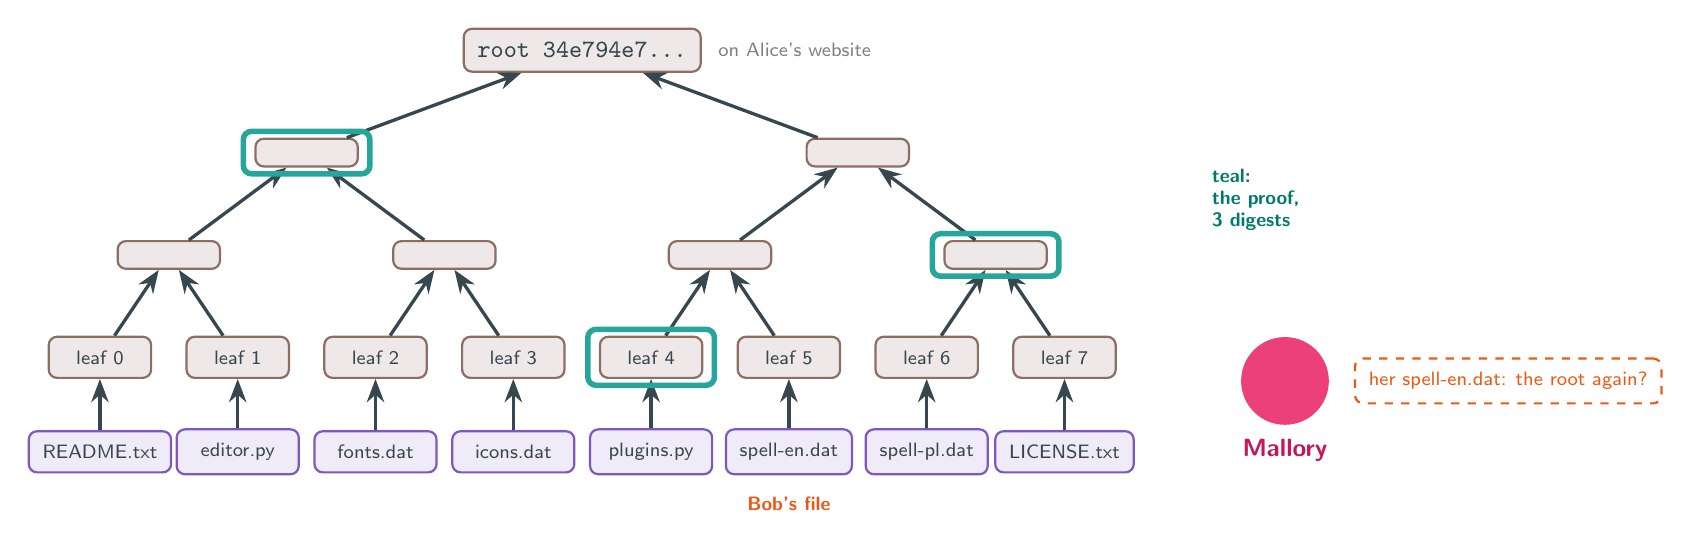
\begin{tikzpicture}[>=Stealth, x=1.75cm]
  \foreach \n [count=\i from 0] in {README.txt, editor.py, fonts.dat, icons.dat, plugins.py, spell-en.dat, spell-pl.dat, LICENSE.txt} {
    \node[msgval, font=\scriptsize, minimum width=1.55cm] (f\i) at (\i,0) {\n};
    \node[dgval, font=\scriptsize, minimum width=1.3cm] (l\i) at (\i,1.2) {leaf \i};
    \draw[data] (f\i) -- (l\i);
  }
  \foreach \j in {0,...,3} {
    \pgfmathsetmacro{\x}{2*\j+0.5}
    \node[dgval, font=\scriptsize, minimum width=1.3cm] (a\j) at (\x,2.5) {};
  }
  \foreach \j in {0,1} {
    \pgfmathsetmacro{\x}{4*\j+1.5}
    \node[dgval, font=\scriptsize, minimum width=1.3cm] (b\j) at (\x,3.8) {};
  }
  \node[dgval, font=\small\ttfamily, minimum width=2.4cm] (r) at (3.5,5.1) {root 34e794e7\ldots};
  \node[font=\scriptsize, text=gray, anchor=west] at (r.east) {\ on Alice's website};
  \foreach \j in {0,...,3} {\pgfmathtruncatemacro{\p}{2*\j}\pgfmathtruncatemacro{\q}{2*\j+1}
    \draw[data] (l\p) -- (a\j); \draw[data] (l\q) -- (a\j);}
  \draw[data] (a0) -- (b0); \draw[data] (a1) -- (b0); \draw[data] (a2) -- (b1); \draw[data] (a3) -- (b1);
  \draw[data] (b0) -- (r); \draw[data] (b1) -- (r);
  \foreach \n in {l4, a3, b0} \draw[sTeal, line width=2pt, rounded corners=3pt] ($(\n.south west)+(-0.08,-0.08)$) rectangle ($(\n.north east)+(0.08,0.08)$);
  \node[font=\scriptsize\bfseries, text=AccentOrange, anchor=north] at (5,-0.45) {Bob's file};
  \node[font=\scriptsize\bfseries, text=sTealText, align=left, anchor=west] at (8.0,3.2) {teal:\\ the proof,\\ 3 digests};
  \mallorynode{mal}{8.6,0.9}
  \node[unk, font=\scriptsize, anchor=west] at (9.1,0.9) {her spell-en.dat: the root again?};
\end{tikzpicture}
\end{document}
